\documentclass[../main.tex]{subfile}

\begin{document}

\section{Численное решение алгебраических уравнений}

Предположим, что нам нужно решить в действительных числах уравнение
$y(x)=0$. Если это просто абстрактное уравнение, то нет единого
алгоритма, как его решить. Первое, что можно сделать -- это локализовать
корни, но это можно сделать лишь по виду функции.

\subsection{Метод бисекции}

Простейший метод отыскания нуля функции -- это метод бисекции, или метод
деления отрезка пополам. Для него нужна лишь совсем небольшая математическая
база.

\begin{algorithm}[метод бисекции]
	Необходимо найти ноль функции $f(x)$ на отрезке $[a,b]$ таком, что:
	\begin{enumerate}[noitemsep, nolistsep]
		\item $f(x)\in C([a,b])$;
		\item $f(a)f(b)<0$, то есть на концах отрезка функция
			принимает значения, противоположные по знаку.
	\end{enumerate}\leavevmode\newline

	Организуем систему вложенных отрезков $[a_n, b_n]$ так, что\\
	$[a_1, b_1]=[a,b]$, а следующие отрезки сформированы следующим образом:
	если $c_k=\frac{a_k+b_k}{2}$, то:
	\begin{itemize}[noitemsep, nolistsep]
		\item Если $f(c_k)=0$, то мы нашли корень, можно не продолжать;
		\item В противном случае, мы берём тот конец отрезка, функция от
			которой не совпала по знаку с $f(c_k)$, и формируем из него
			и точки $c_k$ отрезок $[a_{k+1},b_{k+1}]$.
	\end{itemize}

	Условие выхода: $|f(c_n)|<\varepsilon$, где $\varepsilon>0$ -- некоторая
	погрешность.

	Если данный алгоритм усилить монотонным возрастанием или убыванием на $[a,b]$,
	то ноль на нём будет единственный.
\end{algorithm}

Корректность данного алгоритма напрямую следует из теоремы Больцано-Коши, которая
и доказывается методом бисекции в сочетании с теоремой о двух милиционерах.

\begin{example}
	Пусть нужно решить уравнение
	\[f(x)=x^3-6x^2+8x+2=0.\]

	Функция непрерывна на всей вещественной оси. Значит, с локализацией
	корней проблем быть не должно.
	\newline

	\begin{tabular}{ |c|c|c|c|c| }
		\hline
		$x$		& 0	& 1	& 2	& 3 \\
		\hline
		Знак $f(x)$ 	& $+$	& $+$	& $+$	& $-$ \\
		\hline
	\end{tabular}
	\newline

	%TODO найти команду, которую находит значения функции в точке (параметры: функция и точка)
	Тогда $\exists c\in[2,3]: f(c)=0$. Найдём его методом бисекции:
	\begin{itemize}[noitemsep, nolistsep]
		\item $f(2.5)=0.125>0$, ищем на $[2.5,3]$;
		\item $f(2.75)\approx -0.5781<0$, ищем на $[2.5,2.75]$;
		\item $f(2.625)\approx -0.2259<0$, ищем на $[2.5,2.625]$ и т. д.
	\end{itemize}\leavevmode\newline

	На графике это выглядит вот так:\\

	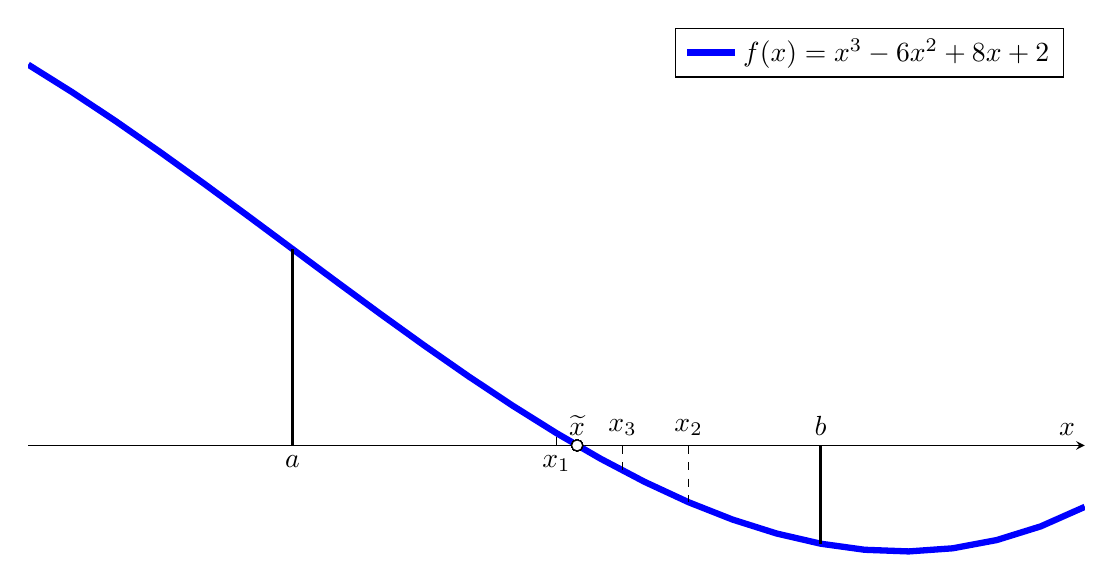
\begin{tikzpicture} [
		declare function={
			f(\x)= \x^3 - 6*\x^2+ 8*\x + 2;
		},
	]
		\begin{axis} [
			height=9cm,
			width=15cm,
			xlabel = {$x$},
			ylabel = {$f(x)$},
			axis x line = middle,
			hide y axis,
			domain = 1.5:3.5,
			ticks = none ]

			\newcommand*{\varA}{2}
			\newcommand*{\varB}{3}
			\newcommand*{\X}{2.539}
			\pgfmathsetmacro{\fb}{f(\varB)}
			\pgfmathsetmacro{\fa}{f(\varA)}
			\pgfmathsetmacro{\Xfirst}{(\varA+\varB)/2}
			\pgfmathsetmacro{\fXfirst}{f(\Xfirst)}
			\pgfmathsetmacro{\Xsecond}{(\Xfirst+\varB)/2}
			\pgfmathsetmacro{\fXsecond}{f(\Xsecond)}
			\pgfmathsetmacro{\Xthird}{(\Xfirst+\Xsecond)/2}
			\pgfmathsetmacro{\fXthird}{f(\Xthird)}

			\addplot[color=blue, line width=.08cm]{f(x)};

			\coordinate(A) at 	(\varA,		\fa);
			\node[below](Ap) at 	(\varA,		0) {$a$};
			\coordinate(B) at 	(\varB,		\fb);
			\node[above](Bp) at 	(\varB,		0) {$b$};
			\node[above](X) at 	(\X,		0) {$\widetilde{x}$};
			\coordinate(X1) at 	(\Xfirst,	\fXfirst);
			\node[below](X1p) at 	(\Xfirst,	0) {$x_1$};
			\coordinate(X2) at 	(\Xsecond,	\fXsecond);
			\node[above](X2p) at 	(\Xsecond,	0) {$x_2$};
			\coordinate(X3) at 	(\Xthird,	\fXthird);
			\node[above](X3p) at 	(\Xthird,	0) {$x_3$};

			\addplot[mark=*,only marks, fill=white] (\X, 0)
				node[above, pos=1]{};

			\draw[very thick] (Ap) -- (A)	(Bp) -- (B);
			\draw[dashed] (X1p) -- (X1)	(X2p) -- (X2)	(X3p) -- (X3);

			\addlegendentry{$f(x)=x^3-6x^2+8x+2$};
		\end{axis}
	\end{tikzpicture}
\end{example}


\subsection{Итерационные методы решения алгебраических уравнений}

Метод бисекции гарантированно даёт нам результат. Но нам бы хотелось иметь
более быструю сходимость. В этом нам могут помочь итерационные методы.

\begin{define}
	\textbf{Итерацией} называется многократное применение одной и той же
	функции $f$ к числу. Пусть задано начальное число $x_0$, тогда:
	\begin{itemize}[noitemsep, nolistsep]
		\item $x_1=f(x_0)$,
		\item $x_2=f(x_1)=f(f(x_0))$,\\
		...
		\item $x_n=f(x_{n-1})=\underset{n}{\underbrace{f(f(...f}}(x_0)...))$.
	\end{itemize}

	\textbf{Последовательность} $\{x_n\}$, образованная таким образом,
	называется \textbf{итерационной} с базой $x_0$ и функцией итерации $f(x)$.
\end{define}

\begin{algorithm}[метод простой итерации]
	Пусть нужно решить уравнение $y(x)=0$. Сделаем подстановку
	$g(x)=x+\tau y(x)$, где $\tau$ -- некоторая положительная константа.
	Таким образом, теперь нужно решить уравнение $g(x)=x$, то есть вместо
	нулей функции мы ищем неподвижные точки.

	Пусть $x_0$ -- некоторое начальное приближение. Построим итерационную
	последовательность с базой $x_0$ и функцией итерации $g(x)$. Если
	параметр $\tau$ подобран правильно, итерационная последовательность
	сойдётся к неподвижной точке. При заданной погрешности $\varepsilon$
	завершаем итерацию при $|g(x_n)-x_n|<\varepsilon$.
\end{algorithm}

Как нужно подобрать $\tau$, чтобы последовательность сошлась? Однозначного ответа
нет. Однако тут частично выручает та теория, которую мы узнали на ДГМА. Дело
идёт о так называемых сжимающих операторах.

Для начала не помешает освежить в своей памяти некоторые определения.

\begin{define}
	\textbf{Метрическим пространством} называется пространство $M$, в
	котором определена операция метрики $\rho: M^2 \rightarrow \mathbb R $
	такая, что $\forall x, y, z \in M$ верно
	\begin{enumerate}[noitemsep, nolistsep]
		\item $\rho(x,y)\ge 0$, причём $\rho(x,y) = 0 \Leftrightarrow x=y$;
		\item $\rho(x,y)=\rho(y,x)$;
		\item $\rho(x,y)\le \rho(x,z) + \rho(z,y)$.
	\end{enumerate}

	Если дополнительно верно, что каждая фундаментальная последовательность
	$M$ сходится к элементу, принадлежащему ему, то $M$ --
	\textbf{полное метрическое пространство}.
\end{define}

\begin{define}
	\textbf{Сжимающим оператором} на метрическом пространстве $M$ с метрикой
	$\rho$ называется оператор $f: M \rightarrow M$ такой, что\\
	$\exists q \in(0;1):\forall x,y \in M\;\; \rho(f(x),f(y)) \le q \rho(x,y)$.

	Число $q$ назовём \textbf{коэффициентом сжатия}.
\end{define}

\begin{theorem}[о сжимающем операторе]
	Пусть $(M,\rho)$ -- полное метрическое пространство, $f$ -- сжимающий
	оператор на $M$ с коэффициентом сжатия $q$. Тогда:
	\begin{enumerate}[noitemsep, nolistsep]
		\item $\exists!\;\widetilde{x}\in M: f(\widetilde{x})=\widetilde{x}$;
		\item Любая последовательность $\{x_n\}$ такая, что $x_0 \in M$ --
			произвольный, $x_{k+1}=f(x_k)$, сходится к $\widetilde{x}$;
		\item Для всякой такой последовательности верно\\
			$\rho(x_n, \widetilde{x}) \le q ^ n \rho(x_0, \widetilde{x})$.
	\end{enumerate}
\end{theorem}

Данная теорема была доказана в курсе "Дополнительные главы математического анализа"{}.
В литературе эта теорема также известна как "Теорема Банаха о неподвижной точке"{}.

Всё это нужно было для того, чтобы доказать красивую, но практически бесполезную
теорему.

\begin{theorem}[о сходимости итерационного процесса]
	Пусть нам необходимо найти неподвижную точку функции $g(x)$. Зададим
	в качестве полного метрического пространства отрезок $G=\{x: |x-a| \le r\}$,
	где $a$ и $r$ -- параметры отрезка. Для того чтобы итерационный процесс
	$x_{k+1}=g(x_k)$ сошёлся, достаточно, чтобы:
	\begin{enumerate}[noitemsep, nolistsep]
		\item $\forall x,y\in G\;|g(x)-g(y)|\le q|x-y|$, где $q\in(0,1)$ --
			некоторая константа, то есть функция непрерывна по Липшицу;
		\item $|g(a)-a|\le(1-q)r$.
	\end{enumerate}
\end{theorem}

\beginproof

	Нам всего лишь нужно доказать, что $g(x)$ замкнута на $G$.
	\begin{multline*}
		\forall x\in G:|g(x)-a|=|g(x)-g(a)+g(a)-a|\le \\
		\le|g(x)-g(a)|+|g(a)-a|.
	\end{multline*}

	Применив условия 1 и 2 к первому и второму модулю соответственно, получаем
	\begin{align*}
		|g(x)-g(a)|+|g(a)-a|\le q|x-a|+(1-q)r\le qr+r-qr=r.
	\end{align*}

	Следовательно, $\forall x\in G: |g(x)-a|\le r\Rightarrow\forall x\in G\;\;g(x)\in G$,
	что и даёт нам замкнутость $g(x)$ на этом отрезке. Условие 1 и замкнутость
	даёт нам право считать $g(x)$ сжимающим отображением, поэтому тут применима
	теорема Банаха о неподвижной точке -- итерационный процесс сходится.\qed\newline

\begin{corollary}
	Пусть функция $f(x)\in C[a,b]=G$, причём $\forall c\in G$ $|f'(c)|<1$,
	а также она замкнута на $G$. Тогда $\exists x\in G: f(x)=x$.
\end{corollary}

\beginproof

	Так как модуль производной ограничен сверху, будем считать, что $|f'(x)|\le q<1$.

	По теореме Лагранжа о среднем значении, $\forall x,y\in G$ \\
	\[\exists z\in[x,y]: f(y)-f(x)=f'(z)(y-x).\]

	Добавим модули: $|f(y)-f(x)|=|f'(z)||y-x|\le q|y-x|$, то есть имеем
	непрерывность по Липшицу, и тогда неподвижная точка на $G$ существует.\qed

\begin{example}[графическая интерпретация метода простой итерации]
	Нужно решить уравнение \(e^x=x+2.\) Как и в предыдущем примере, с
	непрерывностью у данной функции проблем нет.

	Отобразим функции $g(x)=e^x$ и $h(x)=x+2$ на графике:
	\newline

	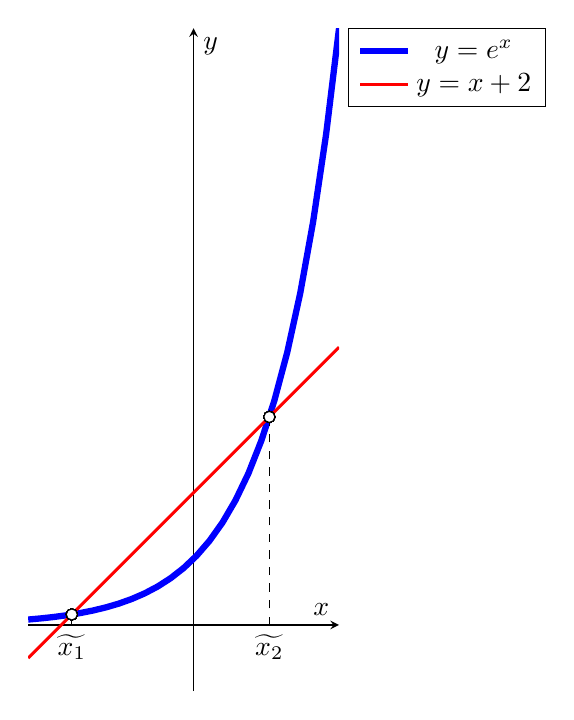
\begin{tikzpicture} [
		declare function = {
			g(\x)=e^\x;
			h(\x)=\x+2;
		},]

		\begin{axis} [
			unit vector ratio*=1 1,
			height=10cm,
			xlabel = {$x$},
			ylabel = {$y$},
			axis x line = middle,
			axis y line = middle,
			domain = -2.5:2.2,
			ymin = -1,
			ticks = none,
			legend pos = outer north east]

			\newcommand*{\Xfirst}{-1.841}
			\newcommand*{\Xsecond}{1.146}
			\pgfmathsetmacro{\fXfirst}{h(\Xfirst)}
			\pgfmathsetmacro{\fXsecond}{h(\Xsecond)}

			\addplot[color=blue, line width=.08cm]{g(x)};
			\addplot[color=red, line width=.04cm]{h(x)};

			\coordinate(X1) at 	(\Xfirst,	\fXfirst);
			\node[below](X1p) at 	(\Xfirst,	0) {$\widetilde{x_1}$};
			\coordinate(X2) at 	(\Xsecond,	\fXsecond);
			\node[below](X2p) at 	(\Xsecond,	0) {$\widetilde{x_2}$};

			\addplot[mark=*,only marks, fill=white] (\Xfirst,\fXfirst)
				node[above, pos=1]{};
			\addplot[mark=*,only marks, fill=white] (\Xsecond,\fXsecond)
				node[above, pos=1]{};

			\draw[dashed] (X1p) -- (X1)	(X2p) -- (X2);

			\addlegendentry{$y=e^x$};
			\addlegendentry{$y=x+2$};
		\end{axis}
	\end{tikzpicture}

	Видно, что у уравнения имеются 2 решения. Обозначим их как $\widetilde{x_1}$
	и $\widetilde{x_2}$. Запишем уравнение так, будто мы ищем нули функции:
	$f(x) = e^x-x-2$. Теперь локализуем корни:
	\newline

	\begin{tabular}{ |c|c|c|c|c|c| }
		\hline
		$x$		& -2	& -1	& 0	& 1	& 2 \\
		\hline
		Знак $f(x)$ 	& $+$	& $-$	& $-$	& $-$ 	& $+$\\
		\hline
	\end{tabular}
	\newline

	$\widetilde{x_1}\in[-2,-1],\;\widetilde{x_2}\in[1,2]$.

	Теперь запишем уравнение через поиск неподвижной точки, то есть как
	$u(x)=e^x-2$.

	Найдём сначала $\widetilde{x_1}$. За начальную точку возьмём $x_1=-1.5$ --
	середину отрезка. Поехали:
	\begin{itemize}[noitemsep, nolistsep]
		\item $x_1=u(-1.5000)\approx -1.7769$, $|u(x_0)-x_0|\approx 0.2769$;
		\item $x_2=u(-1.7769)\approx -1.8308$, $|u(x_1)-x_1|\approx 0.0539$;
		\item $x_3=u(-1.8308)\approx -1.8397$, $|u(x_2)-x_2|\approx 0.0089$ и т. д.
	\end{itemize}

	Итерационная последовательность очень быстро сходится к $\widetilde{x_1}$. Не менее
	интересно будет посмотреть на это на графике:
	\newline

	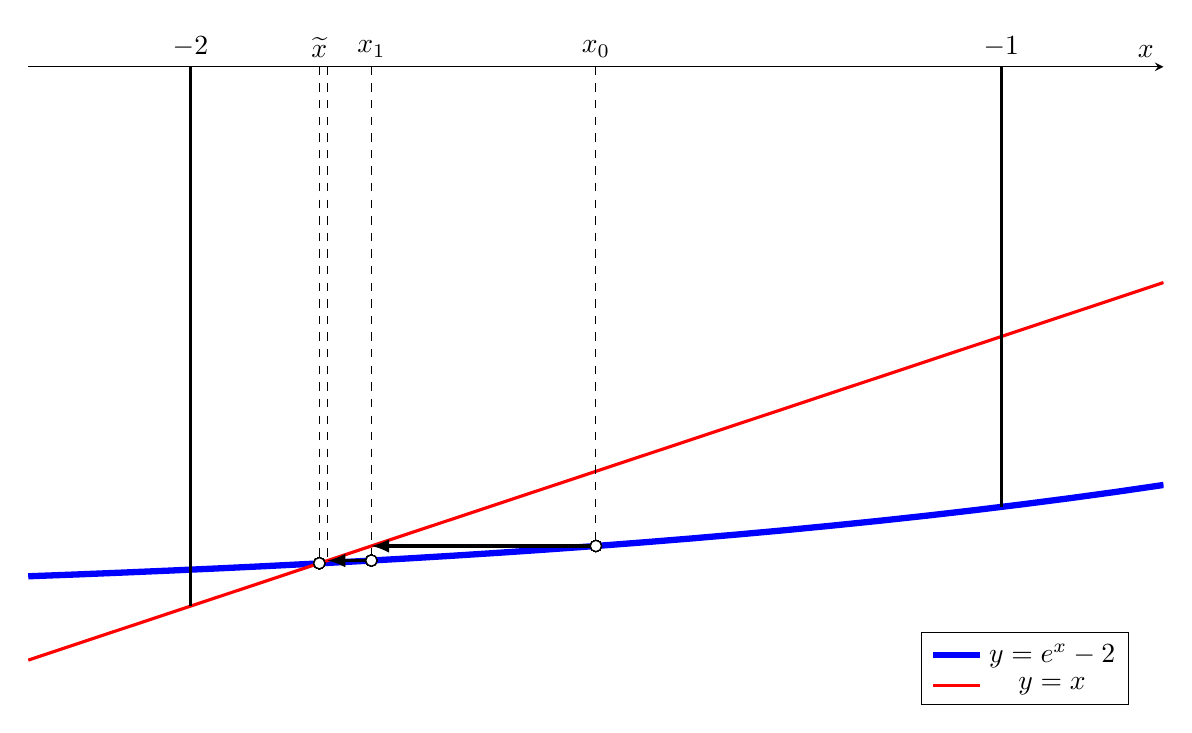
\begin{tikzpicture} [
		declare function= {
			u(\x) = e^\x-2;
			i(\x) = \x;
		},]
		\begin{axis} [
			height=11cm,
			width=16cm,
			xlabel = {$x$},
			ylabel = {$y$},
			axis x line = middle,
			hide y axis,
			ymax = 0.3,
			domain = -2.2:-0.8,
			ticks = none,
			legend pos = south east ]

			\newcommand*{\varA}{-2}
			\newcommand*{\varB}{-1}
			\newcommand*{\trueX}{-1.841}
			\pgfmathsetmacro{\fa}{min(u(\varA), i(\varA))}
			\pgfmathsetmacro{\fb}{min(u(\varB), i(\varB))}
			\pgfmathsetmacro{\Xzeroth}{(\varA+\varB)/2}
			\pgfmathsetmacro{\Xfirst}{(u(\Xzeroth)}
			\pgfmathsetmacro{\Xsecond}{(u(\Xfirst)}
			\pgfmathsetmacro{\Xthird}{(u(\Xsecond)}

			\addplot[color=blue, line width=.08cm]{u(x)};
			\addplot[color=red, line width=.04cm]{i(x)};

			\coordinate(A) at 	(\varA,		\fa);
			\node[above](Ap) at	(\varA,		0) {$\varA$};
			\coordinate(B) at 	(\varB,		\fb);
			\node[above](Bp) at	(\varB,		0) {$\varB$};
			\coordinate(X) at 	(\trueX,	\trueX);
			\node[above](Xp) at	(\trueX,	0) {$\widetilde{x}$};
			\coordinate(X0) at 	(\Xzeroth,	\Xfirst);
			\node[above](X0p) at	(\Xzeroth,	0) {$x_0$};
			\coordinate(X0med) at 	(\Xfirst,	\Xfirst);
			\coordinate(X1) at 	(\Xfirst,	\Xsecond);
			\node[above](X1p) at	(\Xfirst,	0) {$x_1$};
			\coordinate(X1med) at 	(\Xsecond,	\Xsecond);
			\coordinate(X2) at 	(\Xsecond,	\Xthird);
			\coordinate(X2p) at	(\Xsecond,	0);

			\addplot[mark=*,only marks, fill=white] (\trueX,\trueX)
				node[above, pos=1]{};
			\addplot[mark=*,only marks, fill=white] (\Xzeroth,\Xfirst)
				node[above, pos=1]{};
			\addplot[mark=*,only marks, fill=white] (\Xfirst,\Xsecond)
				node[above, pos=1]{};

			\draw[very thick] (Ap) -- (A)	(Bp) -- (B);
			\draw[dashed] (Xp) -- (X)	(X0p) -- (X0)
				(X1p) -- (X1)	(X2p) -- (X2);

			\draw[-latex, very thick] (X0) edge (X0med)
				(X1) -- (X1med);

			\addlegendentry{$y=e^x-2$};
			\addlegendentry{$y=x$};
		\end{axis}
	\end{tikzpicture}
	\newpage

	Теперь попробуем найти $x_2$, который где-то на отрезке $[1,2]$. Как и
	в предыдущем случае, за $x_0$ возьмём середину отрезка, то есть 1.5:
	\begin{itemize}[noitemsep, nolistsep]
		\item $x_1=u(1.5000)\approx 2.4817$, $|u(x_0)-x_0|\approx 0.9817$;
		\item $x_2=u(2.4817)\approx 9.9616$, $|u(x_1)-x_1|\approx 7.4799$;
	\item $x_3=u(9.9616)\approx 21195$ и т. д.
	\end{itemize}

	Вот тут нам не повезло: итерационная последовательность разошлась.
	На это тоже можно посмотреть на графике:
	\newline

	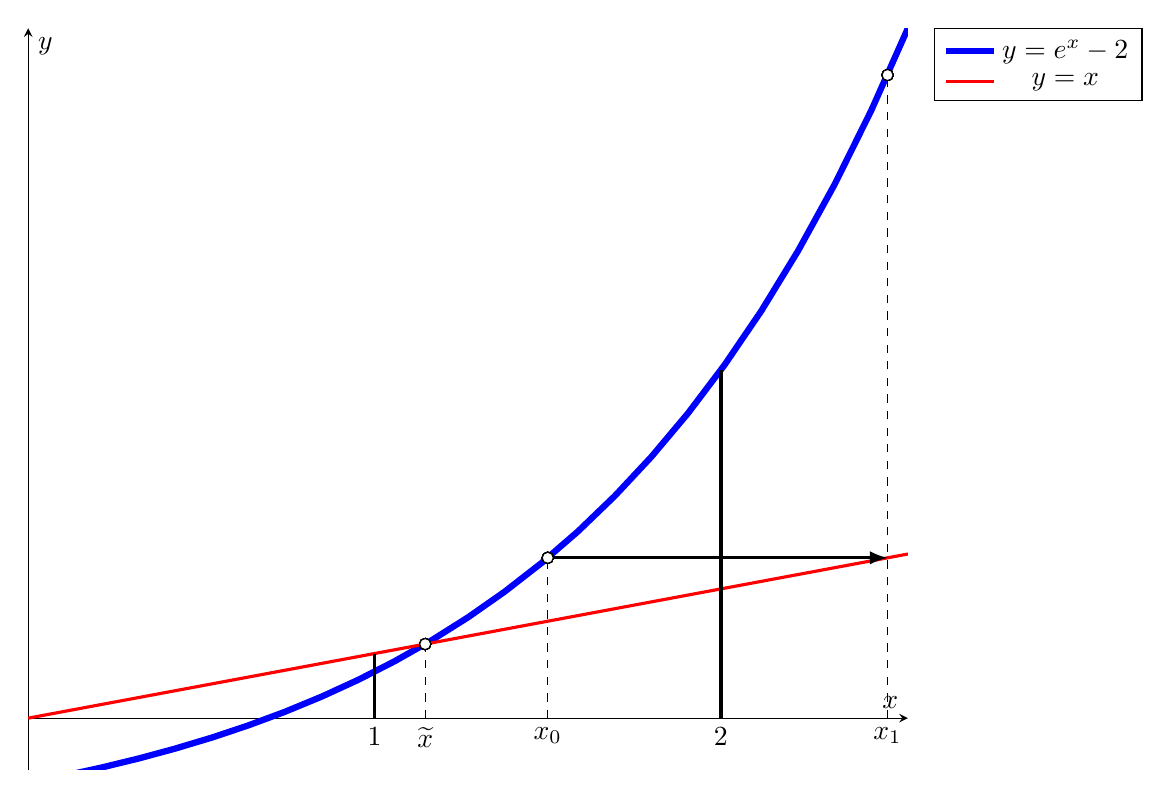
\begin{tikzpicture} [
		declare function= {
			u(\x) = e^\x-2;
			i(\x) = \x;
		},]
		\begin{axis} [
			height=11cm,
			xlabel = {$x$},
			ylabel = {$y$},
			axis x line = middle,
			axis y line = middle,
			ymin = -0.8,
			domain = 0:2.54,
			ticks = none,
			legend pos = outer north east
		]

			\newcommand*{\varA}{1}
			\newcommand*{\varB}{2}
			\newcommand*{\trueX}{1.1462}
			\pgfmathsetmacro{\fa}{max(u(\varA), i(\varA))}
			\pgfmathsetmacro{\fb}{max(u(\varB), i(\varB))}
			\pgfmathsetmacro{\Xzeroth}{(\varA+\varB)/2}
			\pgfmathsetmacro{\Xfirst}{(u(\Xzeroth)}
			\pgfmathsetmacro{\Xsecond}{(u(\Xfirst)}

			\addplot[color=blue, line width=.08cm]{u(x)};
			\addplot[color=red, line width=.04cm]{i(x)};

			\coordinate(A) at 	(\varA,		\fa);
			\node[below](Ap) at	(\varA,		0) {$\varA$};
			\coordinate(B) at 	(\varB,		\fb);
			\node[below](Bp) at	(\varB,		0) {$\varB$};
			\coordinate(X) at 	(\trueX,	\trueX);
			\node[below](Xp) at	(\trueX,	0) {$\widetilde{x}$};
			\coordinate(X0) at 	(\Xzeroth,	\Xfirst);
			\node[below](X0p) at	(\Xzeroth,	0) {$x_0$};
			\coordinate(X0med) at 	(\Xfirst,	\Xfirst);
			\coordinate(X1) at 	(\Xfirst,	\Xsecond);
			\node[below](X1p) at	(\Xfirst,	0) {$x_1$};

			\addplot[mark=*,only marks, fill=white] (\trueX,\trueX)
				node[above, pos=1]{};
			\addplot[mark=*,only marks, fill=white] (\Xzeroth,\Xfirst)
				node[above, pos=1]{};
			\addplot[mark=*,only marks, fill=white] (\Xfirst,\Xsecond)
				node[above, pos=1]{};

			\draw[very thick] (Ap) -- (A)	(Bp) -- (B);
			\draw[dashed]	(Xp) -- (X)	(X0p) -- (X0)
				(X1p) -- (X1);

			\draw[-latex, very thick] (X0) -- (X0med);

			\addlegendentry{$y=e^x-2$};
			\addlegendentry{$y=x$};
		\end{axis}
	\end{tikzpicture}

	Во втором случае расхождение последовательности произошло из-за того, что
	производная $\forall x\ge 1: |u'(x)|>1$.
\end{example}

Однако невыполнение условий теоремы ещё не означает, что итерационная
последовательность не сойдётся к неподвижной точке.

\begin{example}
	Необходимо найти неподвижные точки функции \[f(x)=-e^{2x}+4.5e^x-3.\]

	Предположим, мы уже локализовали одну неподвижную точку на отрезке $[-1,0]$.
	Взяв $x_0$ равным -0.5, начнём строить итерационную последовательность:

	\begin{enumerate}[noitemsep, nolistsep]
		\item $x_1\approx -0.6385, |f(x_0)-x_0|\approx 0.1385$,
		\item $x_2\approx -0.9025, |f(x_1)-x_1|\approx 0.2640$,
		\item $x_3\approx -1.3395, |f(x_2)-x_2|\approx 0.4370$,
		\item $x_4\approx -1.8897, |f(x_3)-x_3|\approx 0.5502$,
		\item $x_5\approx -2.3428, |f(x_4)-x_4|\approx 0.4531$,
		\item $x_6\approx -2.5770, |f(x_5)-x_5|\approx 0.2342$,
		\item $x_7\approx -2.6638, |f(x_6)-x_6|\approx 0.0868$,
		\item $x_8\approx -2.6913, |f(x_7)-x_7|\approx 0.0275$,
		\item $x_9\approx -2.6995, |f(x_8)-x_8|\approx 0.0082$, и т. д.
	\end{enumerate}\leavevmode

	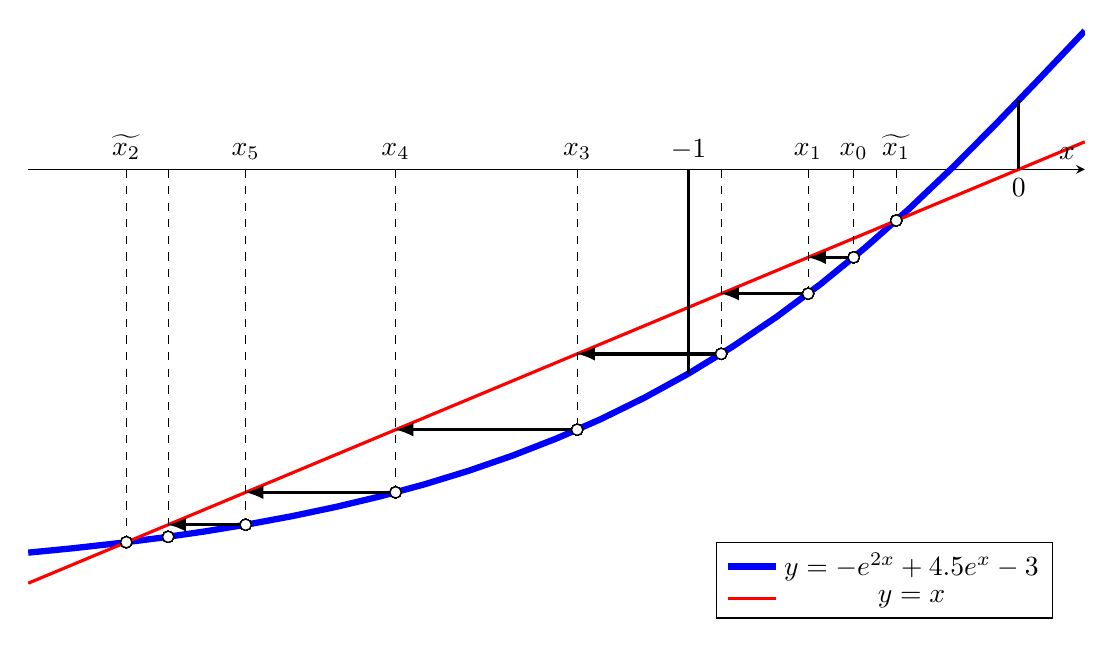
\begin{tikzpicture} [
		declare function= {
			u(\x) = -e^(2*\x) + 4.5 * e^\x - 3;
			i(\x) = \x;
		},]
		\begin{axis} [
			height=10cm,
			width=15cm,
			xlabel = {$x$},
			ylabel = {$y$},
			axis x line = middle,
			hide y axis,
			domain = -3:0.2,
			ticks = none,
			legend pos = south east]

			\newcommand*{\varA}{-1}
			\newcommand*{\varB}{0}
			\newcommand*{\trueXfirst}{-0.371}
			\newcommand*{\trueXsecond}{-2.703}
			\pgfmathsetmacro{\fa}{min(u(\varA), i(\varA))}
			\pgfmathsetmacro{\fb}{max(u(\varB), i(\varB))}
			\pgfmathsetmacro{\Xzeroth}{(\varA+\varB)/2}
			\pgfmathsetmacro{\Xfirst}{(u(\Xzeroth)}
			\pgfmathsetmacro{\Xsecond}{(u(\Xfirst)}
			\pgfmathsetmacro{\Xthird}{(u(\Xsecond)}
			\pgfmathsetmacro{\Xfourth}{(u(\Xthird)}
			\pgfmathsetmacro{\Xfifth}{(u(\Xfourth)}
			\pgfmathsetmacro{\Xsixth}{(u(\Xfifth)}
			\pgfmathsetmacro{\Xseventh}{(u(\Xsixth)}
			\pgfmathsetmacro{\Xeighth}{(u(\Xseventh)}
			\pgfmathsetmacro{\Xnineth}{(u(\Xeighth)}

			\addplot[color=blue, line width=.08cm]{u(x)};
			\addplot[color=red, line width=.04cm]{i(x)};

			\coordinate(A) at 	(\varA,		\fa);
			\coordinate(B) at 	(\varB,		\fb);
			\coordinate(X1true) at 	(\trueXfirst,	\trueXfirst);
			\coordinate(X2true) at 	(\trueXsecond,	\trueXsecond);
			\coordinate(X0) at 	(\Xzeroth,	\Xfirst);
			\coordinate(X1) at 	(\Xfirst,	\Xsecond);
			\coordinate(X2) at 	(\Xsecond,	\Xthird);
			\coordinate(X3) at 	(\Xthird,	\Xfourth);
			\coordinate(X4) at 	(\Xfourth,	\Xfifth);
			\coordinate(X5) at 	(\Xfifth,	\Xsixth);
			\coordinate(X6) at 	(\Xsixth,	\Xseventh);
			\node[above](Ap) at	(\varA,		0) {$\varA$};
			\node[below](Bp) at	(\varB,		0) {$\varB$};
			\node[above](X1trueP)at	(\trueXfirst,	0) {$\widetilde{x_1}$};
			\node[above](X2trueP)at	(\trueXsecond,	0) {$\widetilde{x_2}$};
			\node[above](X0p) at	(\Xzeroth,	0) {$x_0$};
			\node[above](X1p) at	(\Xfirst,	0) {$x_1$};
			\coordinate(X2p) at	(\Xsecond,	0);
			\node[above](X3p) at	(\Xthird,	0) {$x_3$};
			\node[above](X4p) at	(\Xfourth,	0) {$x_4$};
			\node[above](X5p) at	(\Xfifth,	0) {$x_5$};
			\coordinate(X6p) at	(\Xsixth,	0);
			\coordinate(X0med) at 	(\Xfirst,	\Xfirst);
			\coordinate(X1med) at 	(\Xsecond,	\Xsecond);
			\coordinate(X2med) at 	(\Xthird,	\Xthird);
			\coordinate(X3med) at 	(\Xfourth,	\Xfourth);
			\coordinate(X4med) at 	(\Xfifth,	\Xfifth);
			\coordinate(X5med) at 	(\Xsixth,	\Xsixth);

			\addplot[mark=*,only marks, fill=white] (\trueXfirst, \trueXfirst)
				node[above, pos=1]{};
			\addplot[mark=*,only marks, fill=white] (\trueXsecond, \trueXsecond)
				node[above, pos=1]{};
			\addplot[mark=*,only marks, fill=white] (\Xzeroth,\Xfirst)
				node[above, pos=1]{};
			\addplot[mark=*,only marks, fill=white] (\Xfirst,\Xsecond)
				node[above, pos=1]{};
			\addplot[mark=*,only marks, fill=white] (\Xsecond,\Xthird)
				node[above, pos=1]{};
			\addplot[mark=*,only marks, fill=white] (\Xthird,\Xfourth)
				node[above, pos=1]{};
			\addplot[mark=*,only marks, fill=white] (\Xfourth,\Xfifth)
				node[above, pos=1]{};
			\addplot[mark=*,only marks, fill=white] (\Xfifth,\Xsixth)
				node[above, pos=1]{};
			\addplot[mark=*,only marks, fill=white] (\Xsixth,\Xseventh)
				node[above, pos=1]{};

			\draw[very thick] (Ap) -- (A)		(Bp) -- (B);
			\draw[dashed] (X1trueP) -- (X1true)	(X2trueP) -- (X2true)
				(X0p) -- (X0)	(X1p) -- (X1)	(X2p) -- (X2)
				(X3p) -- (X3)	(X4p) -- (X4)	(X5p) -- (X5)
				(X6p) -- (X6);

			\draw[-latex, very thick] (X0) edge (X0med) (X1) edge (X1med)
				(X2) edge (X2med) (X3) edge (X3med) (X4) edge (X4med)
				(X5) -- (X5med);

			\addlegendentry{$y=-e^{2x}+4.5e^x-3$};
			\addlegendentry{$y=x$};
		\end{axis}
	\end{tikzpicture}

	С другой стороны, итерационная последовательность сошлась к числу не из
	нашего отрезка.
\end{example}

\subsection{Метод Ньютона}

Одним из самых эффективных численных методов решения нелинейных уравнений на
отрезке $[a,b]$ вида $f(x)=0$ является метод Ньютона, он же метод касательных.
Здесь будет испозьзована линеаризация уравнения, которая сводит решение
нелинейной задачи к решению последовательности линейных задач.

\begin{algorithm}[метод Ньютона]
	Пусть для уравнения $f(x)=0$ построено приближение $x_k$ к корню
	$\widetilde{x}$. Представим функцию $f(x)$ в окрестности точки $x_k$ в
	виде ряда Тейлора:
	\[f(x)=f(x_k)+f'(x_k)(x-x_k)+\frac{f''(x_k)}{2!}(x-x_k)^2+...\;.\]

	Возьмём от уравнения только линейную часть и положим \\
	$f(x)=0$. Тогда мы имеем:
	\[f(x_k)+f'(x_k)(x-x_k)=0.\]

	Положив решение уравнения относительно $x$ новым приближением к
	$\widetilde{x}$ и обозначением $x_{k+1}$, мы получили следующую формулу:
	\[\boxed{x_{k+1}=x_k-\frac{f(x_k)}{f'(x_k)}.}\]
\end{algorithm}

Теперь не помешало бы определить область задач, где метод Ньютона применим.
\newline

\begin{theorem}[условие сходимости метода Ньютона]
	Пусть $f(x)$ на отрезке $[a,b]=G$ обладает следующими свойствами:
	\begin{enumerate}[noitemsep, nolistsep]
		\item $f(x)\in C^2(G)$;
		\item $f(a)f(b)<0$;
		\item $f'(x)$ и $f''(x)$ отличны от нуля и знакопостоянны на $G$;
		\item Для начального приближения $x_0\in G$ верно $f(x_0)f''(x_0)>0$.
	\end{enumerate}

	Тогда у функции существует единственный ноль $\widetilde{x}$ на $G$, а
	итерационная последовательность $\{x_n\}$, построенная по методу Ньютона,
	\underline{монотонно} сходится к нему.
\end{theorem}

\beginproof

	Из условий 2 и 3 по теореме Больцано-Коши мы сразу получаем существование
	и единственность нуля функции $\widetilde{x}\in G$.

	Далее, для определённости будем считать, что
	\[f(a)<0, f(b)>0,\;\forall x\in G f'(x)>0, f''(x)>0.\]

	Доказательство для второго случая аналогичное.

	В рассматриваемом случае, из условия 4 $f(x_0)>0$, можем взять конкретно
	$x_0=b$. Теперь методом математической индукции докажем, что
	$\forall n\in \mathbb N\;\;x_n>\widetilde{x}$.

	Для $x_0=b$ это тривиально, так как функция возрастающая.

	Теперь положим, что верно $x_k>\widetilde{x}$. Покажем, что для $k+1$
	это тоже верно.

	Положив, что $z_k\in[\widetilde{x},x_k]$, разложим в ряд Тейлора:
	\[0=f(\widetilde{x})=f(x_k)+f'(x_k)(\widetilde{x}-x_k)+
		\underset{>0}{\underbrace{\frac{f''(z_k)}
		{2}(\widetilde{x}-x_k)^2}}.\]

	Откинув последнее слагаемое, получаем:
	\[f(x_k)+f'(x_k)(\widetilde{x}-x_k)<0\Rightarrow
		\widetilde{x}<\underset{x_{k+1}}{
			\underbrace{x_k-\frac{f(x_k)}{f'(x_k)}}}.\]

	Из этого же неравенства вытекает $x_{k+1}<x_k$. Тогда последовательность
	$\{x_n\}$ имеет предел $\overline{x}$, поскольку она монотонно убывает и
	ограничена снизу. Перейдём к пределу в формуле метода Ньютона:
	\[\overline{x}=\overline{x}-\frac{f(\overline{x})}{f'(\overline{x})}
		\Rightarrow f(\overline{x})=0\Rightarrow \overline{x}=
		\widetilde{x}.\]\qed

На словах нельзя утверждать, что метод Ньютона очень эффективен. Чтобы проверить
его на деле, нужно узнать, как быстро уменьшается отклонение от искомого нуля
функции.

Сначала дадим общую оценку.

\begin{lemma}
	Пусть $\widetilde{x}$ и $\overline{x}$ -- точный и приближённый корни
	уравнения $f(x)=0$ на отрезке $[a,b]$ соответственно, сама функция $f(x)$
	такая, что \\ $\forall x\in[a,b]\;\;|f'(x)|\ge m_1>0$. Тогда верно неравенство
	\[|\overline{x}-\widetilde{x}|\le\frac{|f(\overline{x})|}{m_1}.\]
\end{lemma}

\beginproof

	Из существования производной следует непрерывность функции, тогда применима
	теорема Лагранжа о среднем:
	\[f(\overline{x})-f(\widetilde{x})=f'(z)(\overline{x}-\widetilde{x}),\]
	где $z\in[\overline{x},\widetilde{x}]\subseteq[a,b]$. Добавим модулей:
	\[|f(\overline{x})-\underset{=0}{\underbrace{f(\widetilde{x})}}|=|f'(z)|
		|\overline{x}-\widetilde{x}|\ge m_1|\overline{x}-\widetilde{x}|\Rightarrow
		|\overline{x}-\widetilde{x}|\le\frac{|f(\overline{x})|}{m_1}.\]\qed

\end{document}
